\documentclass[aspectratio=169, 10pt]{beamer}

\usepackage[utf8]{inputenc}
\usepackage[T1]{fontenc}
\usepackage[spanish,mexico]{babel}
\usepackage{amsmath, amsthm, amssymb}
\usepackage{hyperref}
\usepackage{graphicx}

\usepackage{float}
\usepackage{animate}
\usepackage{subcaption}
\usepackage{multicol}
\usepackage{verbatim}
\usepackage{xcolor}
\usepackage{listings}
\usepackage{ragged2e}


\usepackage{transparent}

%\usepackage[latin1]{inputenc}
\usepackage[normalem]{ulem}
\usepackage{pifont}
\usepackage{parskip}

\usepackage[all]{xy}

\usetheme{Warsaw} % Warsaw, Bergen, Madrid, CambridgeUS, Berlin, Antibes 
\usecolortheme{seahorse} %albatross, beaver, crane, wolverine, seahorse
\title[\hspace{25mm} \insertframenumber/\inserttotalframenumber]{\bf \Large{Introducción a Latex}}
\subtitle{Clase 1}
%\author[Miguel Ángel Carrillo Lucía]{Ing. Miguel~Ángel~Carrillo~Lucía\inst{1,2}}

\author[Taller de Herramientas Computacionales - 2024-1] % (optional, for multiple authors)
{\hspace{2.70mm} \Large{Miguel Ángel Carrillo Lucía }  \and \Large{Leonard David Solís Rodríguez}} %\inst{1}}

%% Institución
\institute[] % no es necesario llenar la opción
{	{\large Universidad Nacional Autónoma de Mexico}\\
    {\large Facultad de Ciencias}\\
    {\large Departamento de Matemáticas}\\
    {\large Licenciatura en Matematicas Aplicadas}
}
%\institute{Ciudad de México}
\date{14 de agosto de 2025}

\usepackage{transparent}
\usepackage{eso-pic}

%\setbeamertemplate{background}{

%{\transparent{0.075}\includegraphics[width=1.0\paperwidth,height=1.0\paperheight]{escudos/matematicas_aplicadas.jpg}}
%}


\setbeamertemplate{background}{
  \rule{0pt}
  {.90\paperheight}%
  %{0.90}\paperheight
  \hspace*{.5\paperwidth}%
  \paperwidth1.50mm
  \makebox[1pt][c]{\transparent{0.120}
\includegraphics[scale=0.56]{logos_unam_ciencias.png}}
}

%\setbeamertemplate{background}{
%  \hspace*{.5\paperwidth}%
%  \makebox[1pt][c]{%
%    {\transparent{0.2}
\includegraphics[scale=0.56]{logos_unam_ciencias.png}}%
%  }%
%}


\setlength{\columnseprule}{1.5pt}
\def\columnseprulecolor{\color{blue}}

\begin{document}

%\maketitle

\begin{frame}
    \titlepage
    %\vspace{-50pt}
    %\begin{figure}[htpb]
    %    \begin{center}
    %        \includegraphics[width=0.145\linewidth]{escudos/escudo_ciencias_unam.png} \hspace{95mm}
    %        \includegraphics[width=0.145\linewidth]{escudos/escudo_unam.png}
    %    \end{center}
    %\end{figure}
\end{frame}

%\section{Agenda}

%\section{Agenda}
\begin{frame}{Agenda}
     \tableofcontents[sectionstyle=show,subsectionstyle=show/shaded/hide,subsubsectionstyle=show/shaded/hide]
\end{frame}


%%% breve historia de latex

\begin{frame}{Breve historia de Latex}
\begin{columns}
    \begin{column}{.28\linewidth}
        %\begin{exampleblock}{}
        \begin{itemize}
        \justifying
        \begin{figure}
                \centering
                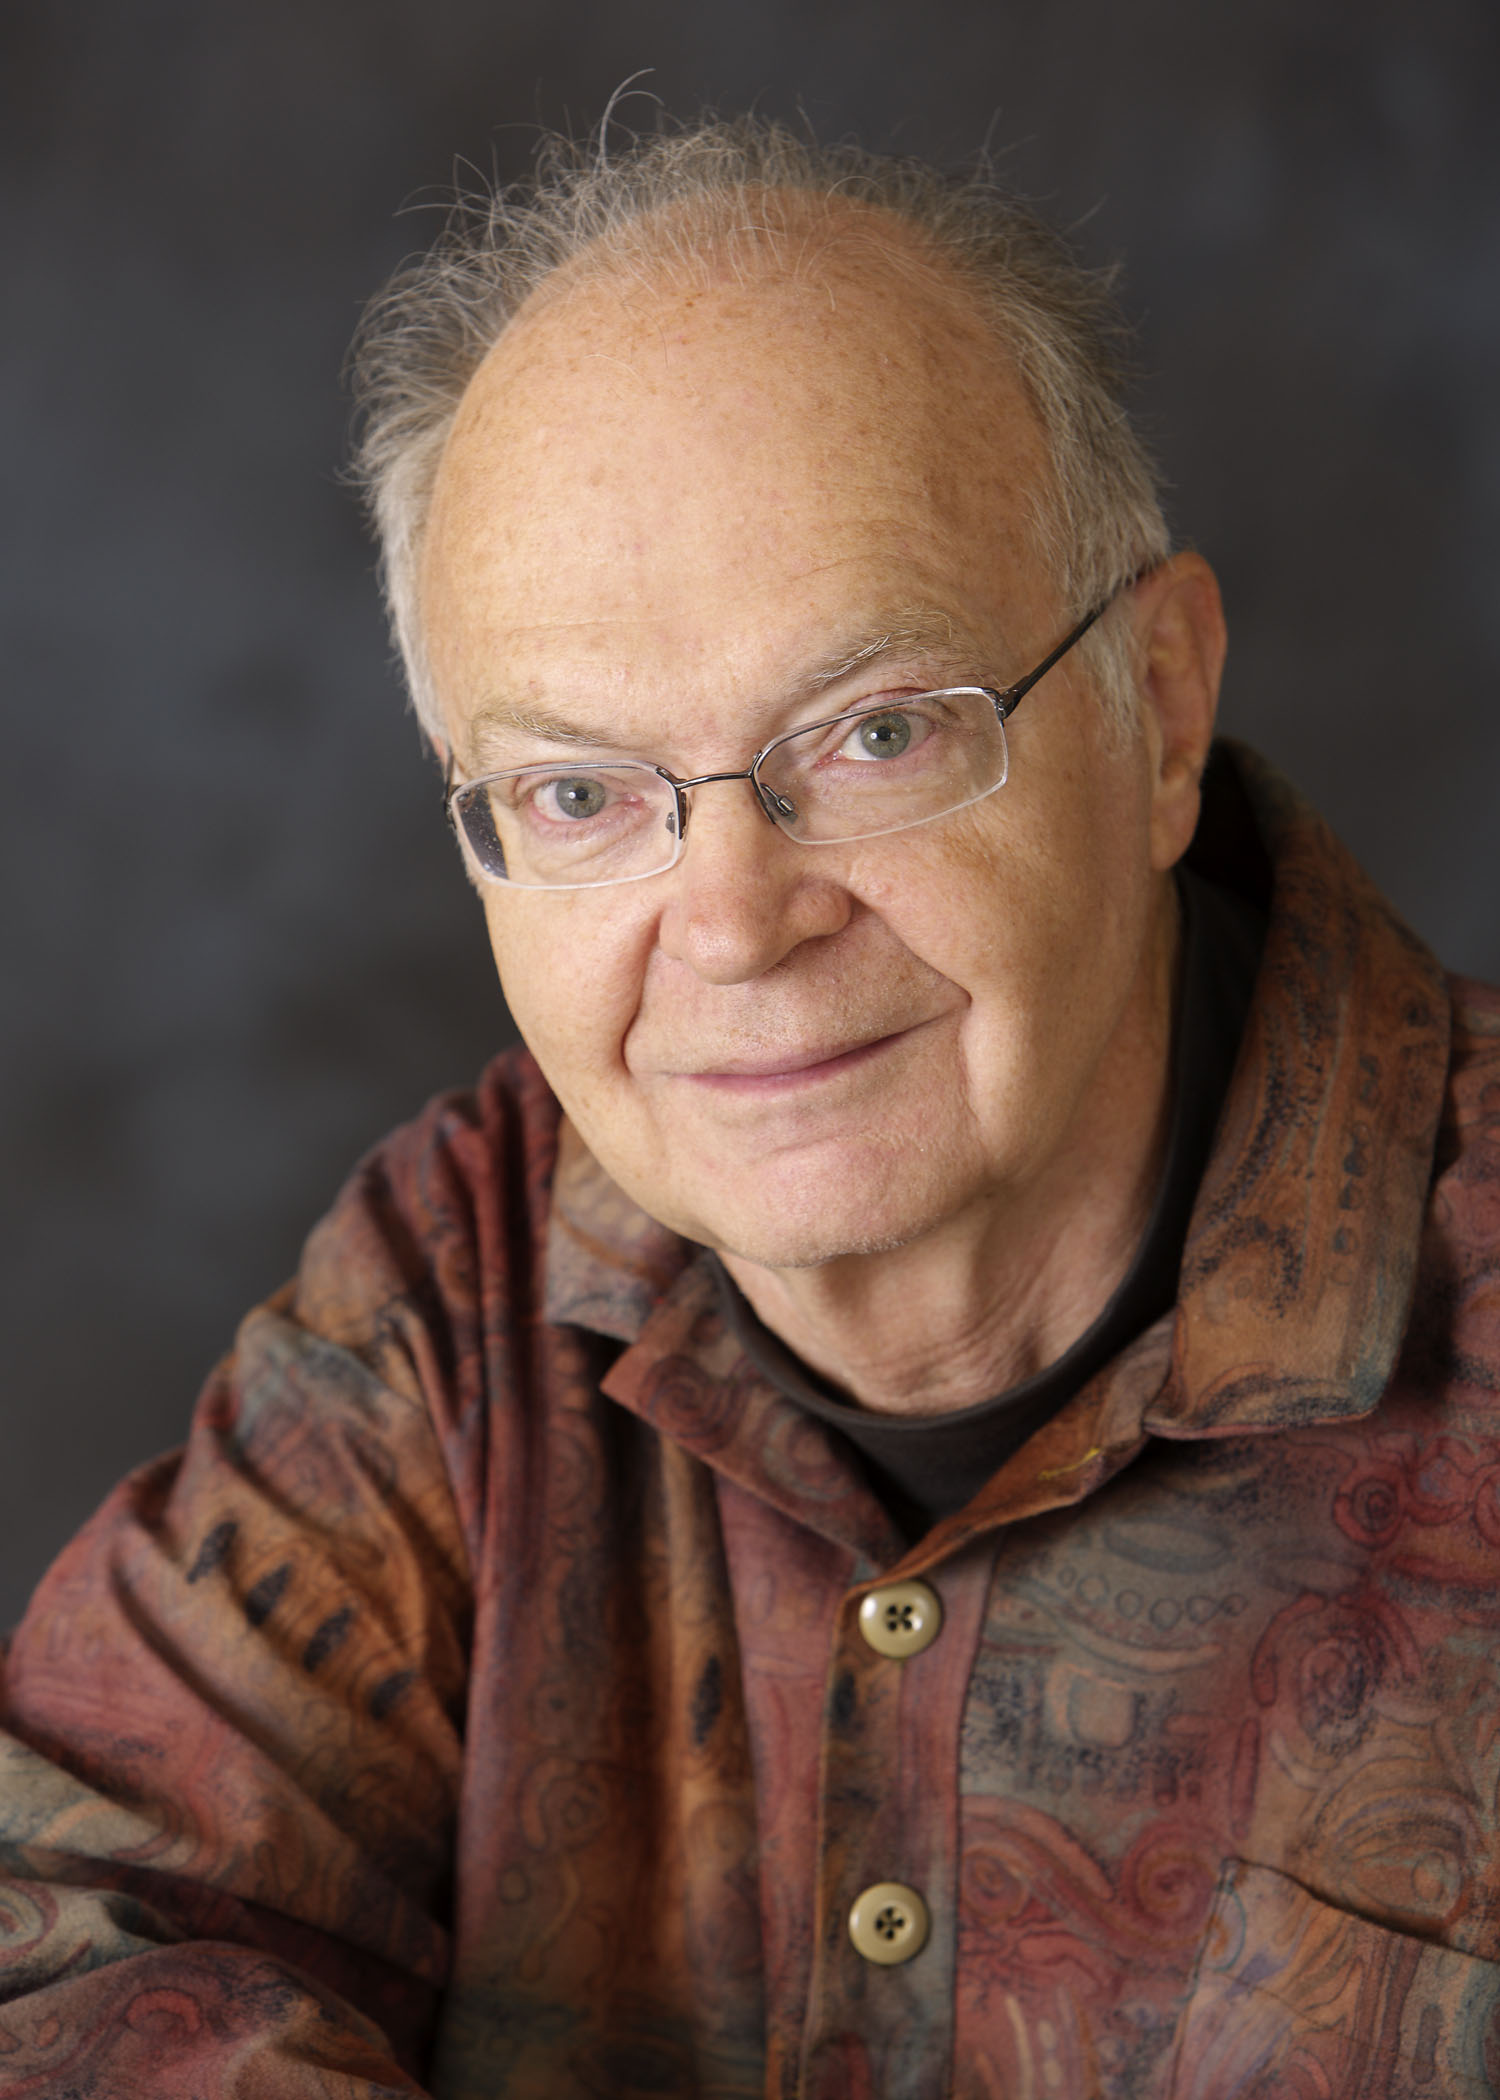
\includegraphics[scale=0.20]{Knuth_donald.jpg} 
               \hspace{-8mm} \caption*{Donald Knuth.}
                \label{}
        \end{figure}    
            %\item TEX: creado por Donald Knuth (1970) como un programa para procesar textos con enfoque al contenido y no a la forma. Define la estructura y tipografía para cada tipo de documento. Es un lenguaje de bajo nivel.
    \end{itemize}
        %\end{exampleblock}
    \end{column}

    \begin{column}{.28\linewidth}
        %\begin{exampleblock}{}
            \begin{itemize}
            \justifying
            \begin{figure}
                \centering
                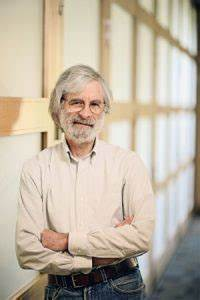
\includegraphics[scale=0.32]{LeslieLamport.jpg} 
                \hspace{-8mm} \caption*{Leslie Lamport.}
                \label{}
            \end{figure}    
                
                %\item En el año 1983 Leslie Lamport en 1983 desarrolla el sistema \LaTeX para facilitar al usuario generar un proyecto (sin preocuparse por la tipografía, márgenes, distribución de texto) mediante una serie de macros. Más fácil de usar.
            \end{itemize}
        %\end{exampleblock}   
    \end{column}
\end{columns}

\vspace{-5mm} \pause
        \begin{alertblock}{¿Qué es un macro?}
            \begin{itemize}
            \justifying
                \item Un macro es un código fuente muy grande para conseguir que el texto generado tenga alguna característica deseada.
            \end{itemize}
        \end{alertblock}
    
\end{frame}

\section{¿Qué es \LaTeX}

\begin{frame}{¿Qué es \LaTeX ?}
    \begin{itemize}
    \justifying
        \item Un sistema de composición de textos que permite obtener fácilmente resultados de calidad profesional. Está orientado al ámbito científico. Permite generar documentos profesionales con alta calidad tipográfica.
        \item Es un lenguaje de programación orientado a generar textos. 
        %\item No solo es procesador de textos sino un lenguaje de programación orientado a su generación.
        \item Está compuesto por un conjunto de Macros  que incorporan una serie de estilos de documentos (libros, artículos, presentaciones, etc.) con características de generación automática.%(programas, bloques de código, que definen instrucciones complejas a partir de otras más simples)
        \item En 1991 se resuelven los problemas de portabilidad, código ASCII (longitud de palabra limitada), UTF-8 (de Unicode Transformation Format) e idiomas. Actualmente, la paquetería UTF-8 ya no se incluye.
        %\item lenguaje que nos permite preparar automáticamente un documento de apariencia estándar y de alta calidad.
    \end{itemize}

\end{frame}

\subsection{Entonces ¿Qué es y qué no es \LaTeX?}
\begin{frame}{Entonces ¿Qué es y qué no es \LaTeX?}
    \begin{itemize}
    \justifying
        \item No es un procesador de textos.
        \item Permite preparar textos que no se editan de manera habitual (viendo el producto), sino que se programan atendiendo más bien a la organización lógica de las ideas.
        \item No es un sistema WYSIWYG (What You See Is What You Get). Lo que ves es lo que hay, o lo que obtienes. ¿Qué significa? 
        \item WYSIWYM (What You See Is What You Mean) lo que ves es lo que quieres decir.
        %\item Es un sistema tipográfico multiplataforma, basado en un lenguaje de descripción de páginas o de marcas.
    \end{itemize}
\end{frame}


\subsection{Estructura. Características}
\begin{frame}{Estructura. Características.}

\begin{itemize}
    \item \LaTeX es un sistema de tipografía diseñado para la composición de textos científicos, tales como:
    \vspace{5mm} \pause
    
\begin{columns}
    \begin{column}{.16\linewidth}
    \centering
    Artículos
    \begin{figure}[H]
        \centering
        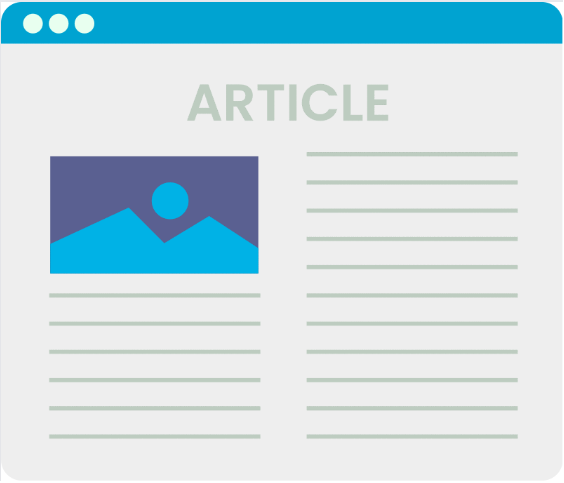
\includegraphics[scale=.1]{article.png} 
        %\caption{Artículo}
        %\label{fig:enter-label}
    \end{figure}
    \end{column} \pause

    \begin{column}{.16\linewidth}
    \centering
    Informes
    \begin{figure}[H]
        \centering
        
\includegraphics[scale=.1]{informe.png} 
        %\caption{Informe}
        %\label{fig:enter-label}
    \end{figure}
    \end{column} \pause

    \begin{column}{.16\linewidth}
    \centering
    Libro
    \begin{figure}
        \centering
        
\includegraphics[scale=.1]{libro.png} 
        %\caption{Libro}
        \label{fig:enter-label}
    \end{figure}
    \end{column} \pause
    
    \begin{column}{.16\linewidth}
    \centering
    Tesis
    \begin{figure}
        \centering
        
\includegraphics[scale=.1]{tesis.png} 
        %\caption{Tesis}
        \label{fig:enter-label}
    \end{figure}
    \end{column} \pause
    
    \begin{column}{.14\linewidth}
    \centering
    Presentaciones
    \begin{figure}[H]
        \centering
        
\includegraphics[scale=.1]{ppt.png} 
        %\caption{Presentaciones}
        %\label{fig:enter-label}
    \end{figure}
    \end{column} \pause
    
\end{columns}    
    
    %\begin{itemize}
    %    \item Artículos
    %    \item Informes
    %    \item Libros
    %    \item Tesis
    %    \item Presentaciones
    %    \item Poster e Infografías.
    %\end{itemize}
    \item Muy útil para publicaciones de interés científico (ingeniería, biología, matemáticas, etc.). \pause
\end{itemize}
    
    \begin{alertblock}{Recuerde} \pause
        \begin{itemize}
        \justifying
            \item \LaTeX no es un procesador de textos (es solo una parte en la generación del documento). \pause
            \item \LaTeX es un lenguaje de programación que nos permite preparar automáticamente un documento de apariencia estándar y de alta calidad.
        \end{itemize}
    \end{alertblock}
\end{frame}

\begin{frame}{Esquema de funcionamiento}

   \begin{figure}
        \centering
       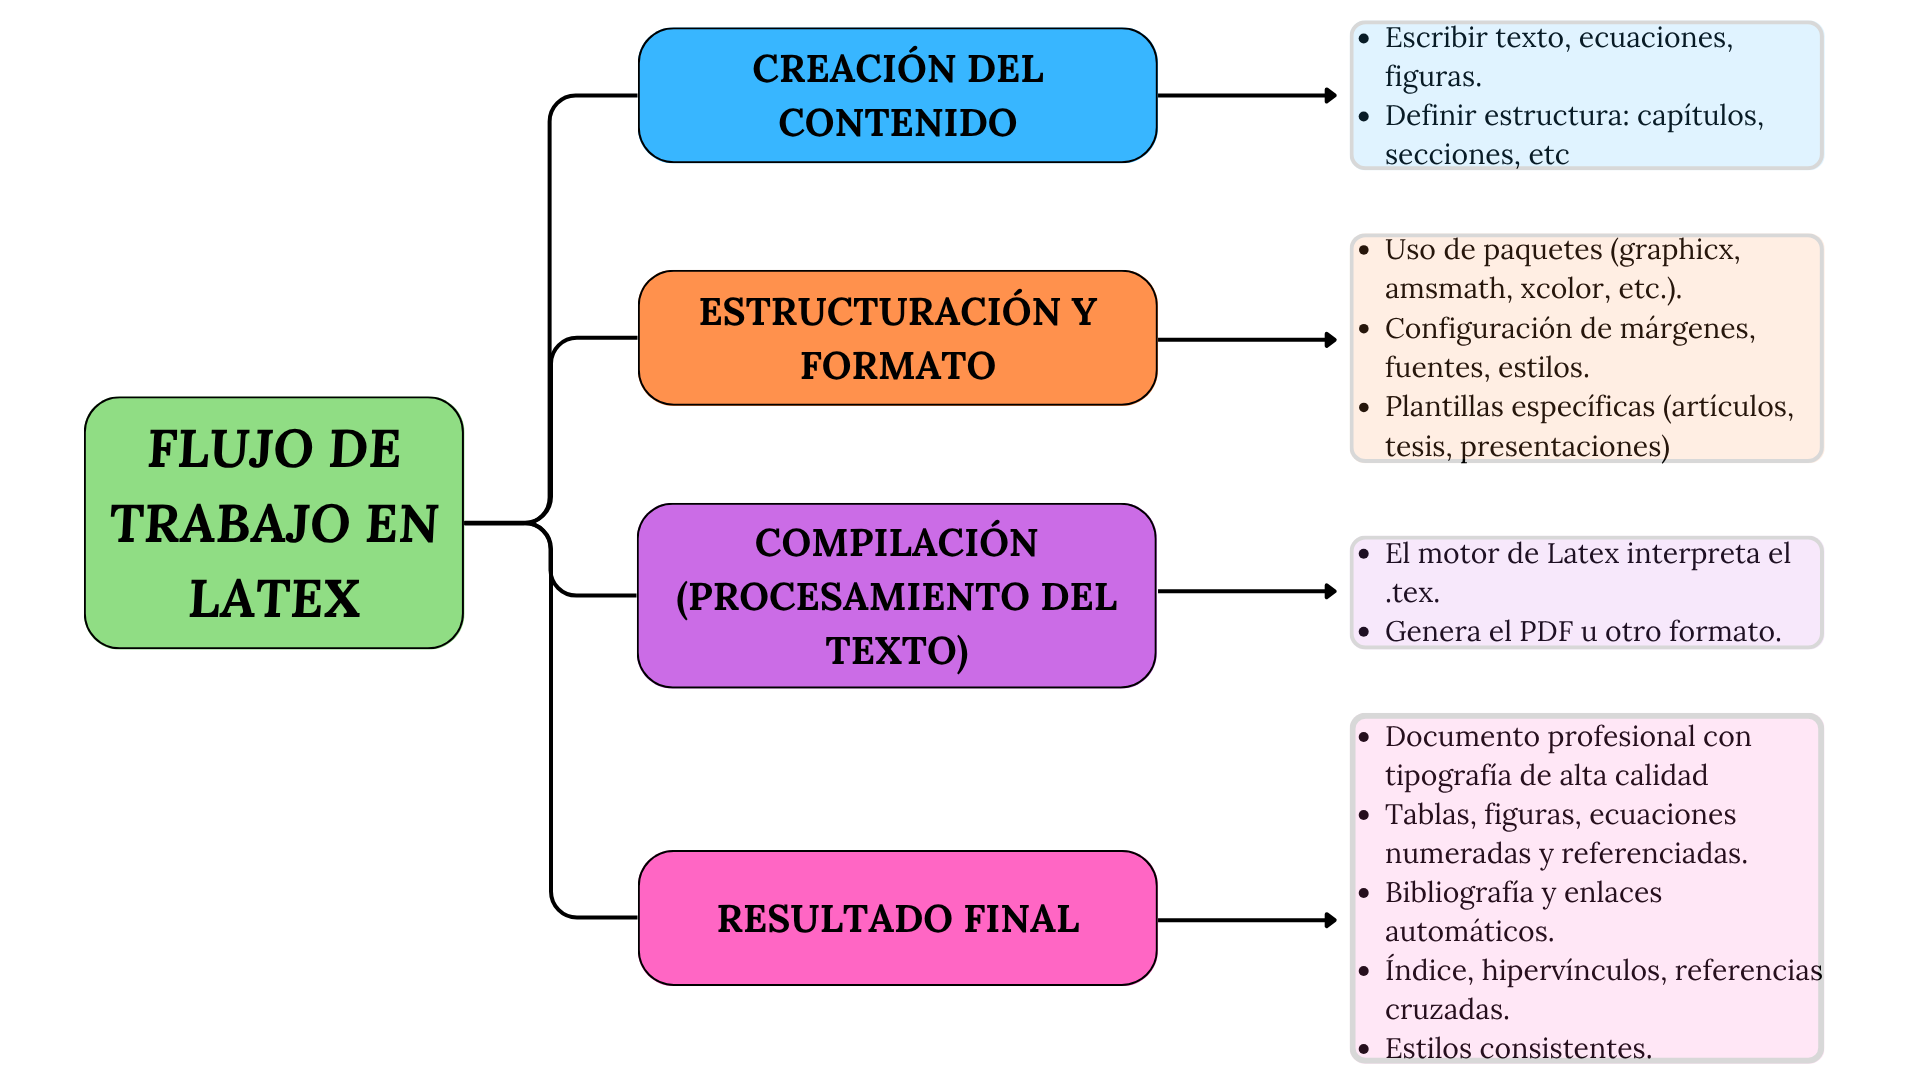
\includegraphics[scale=0.23]{9.png} 
        \caption{Esquema de func.}
        \label{fig:9}
    \end{figure}
\end{frame}

\begin{frame}{Esquema de funcionamiento}

   \begin{figure}
        \centering
        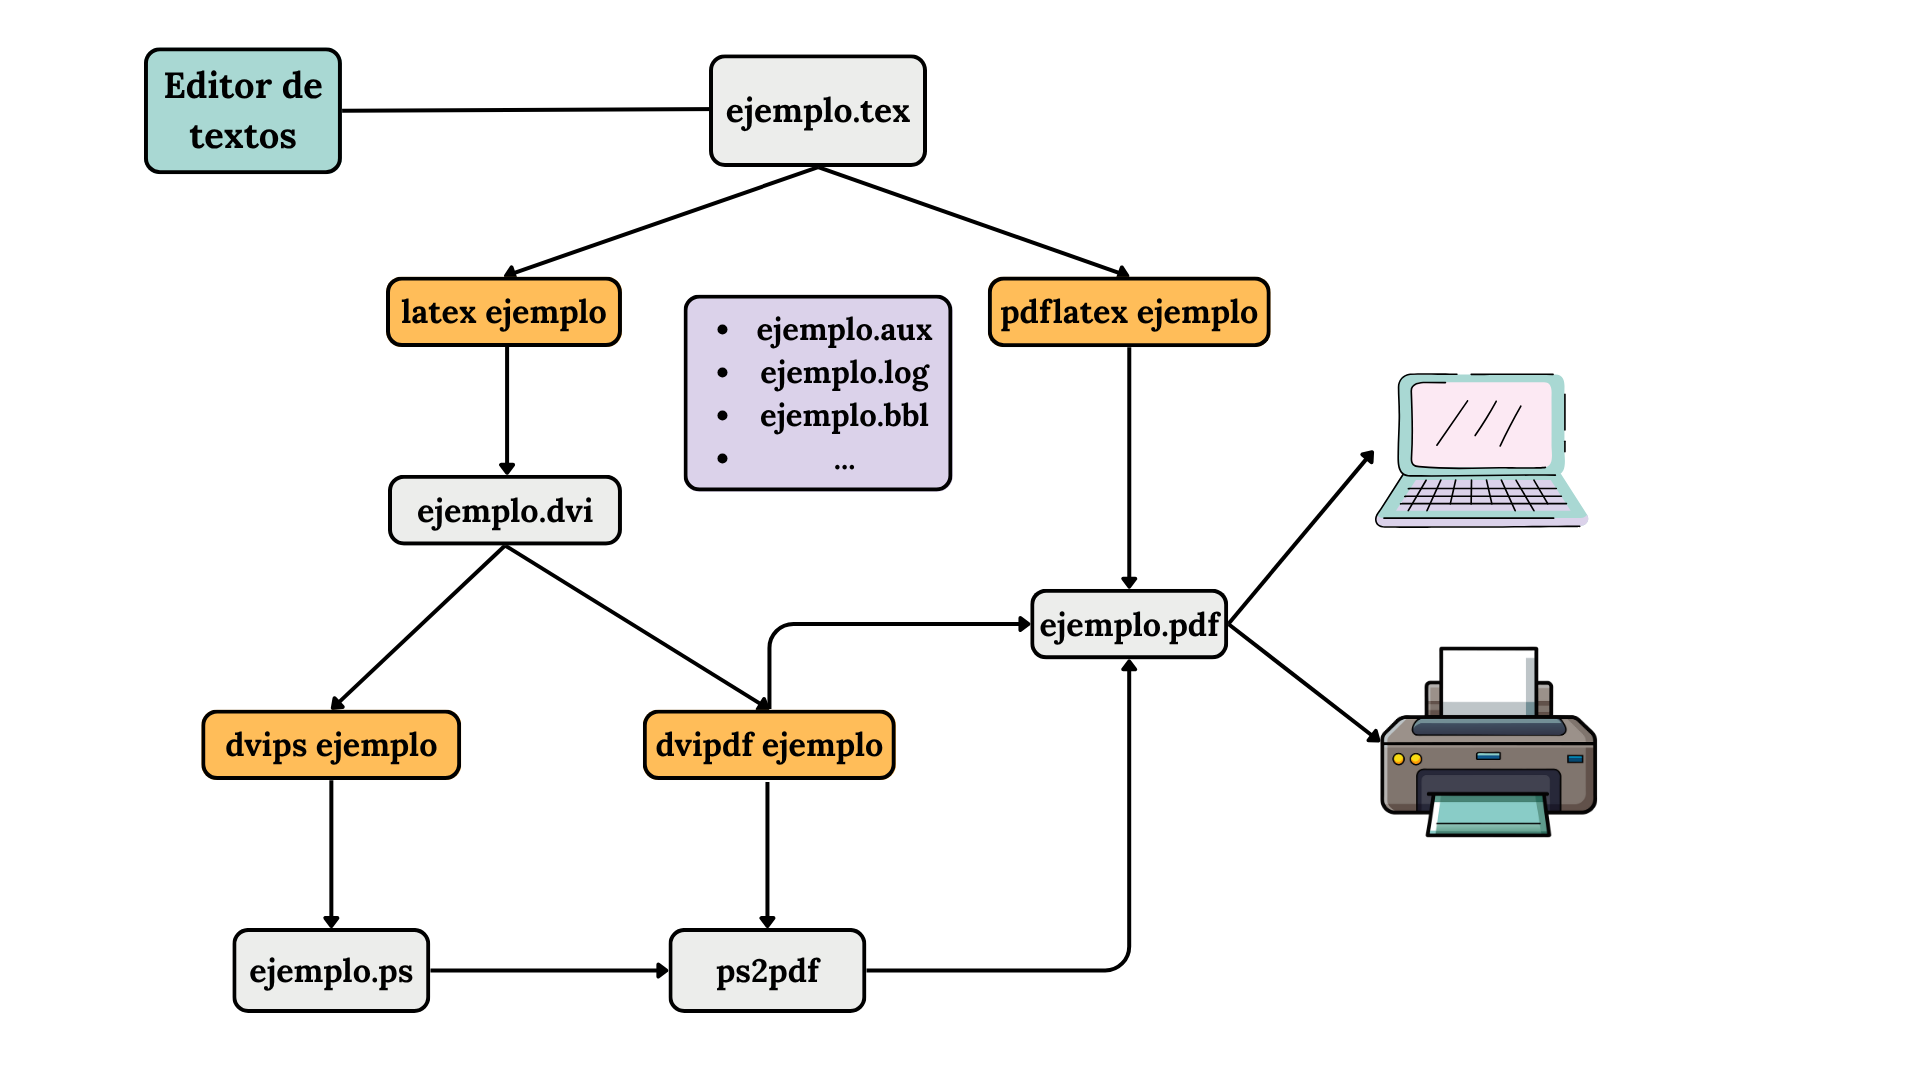
\includegraphics[scale=0.24]{FlujoLatex.png} 
        
        \label{fig:10l}

    \end{figure}
\end{frame}

\subsection{Ventajas y desventajas}
\begin{frame}{Ventajas y desventajas}
\begin{columns} 
    \begin{column}{.48\linewidth}
        \begin{exampleblock}{Ventajas}
        \pause
            \begin{enumerate}
            \item Es gratuito y abierto.
            \item Los documentos son de muy buena calidad tipográfica. 
            \item Portabilidad.
            \item Estabilidad en la forma del documento. 
            \item Automatización de la estructura del documento.
            \item Estilo de trabajo WYSIWYM (diferente a WYSIWYG). 
            \item \LaTeX se encarga del formato y usted del contenido.
    \end{enumerate}
        \end{exampleblock}
        
    \end{column}

    \begin{column}{.48\linewidth} \pause
    \vspace{-5.5mm}
        \begin{exampleblock}{Desventajas} \pause
            \begin{enumerate}
                \item Indicar la estructura lógica del documento (títulos, secciones, subsecciones, pies de páginas).
                \item Las instrucciones deben ser muy concretas sobre las características del formato. 
                \item La información debe ser precisa para que el sistema lo entienda. 
                \item Manejo de errores y advertencias. 
                \item No hay revisor ortográfico.
            \end{enumerate}
        \end{exampleblock}
        
    \end{column}
\end{columns}
    
\end{frame}

\begin{frame}{Opciones de escritorio}
\begin{figure}
    \centering
    \begin{minipage}{0.10\textwidth}
        
\includegraphics[scale=0.040]{lyx.png} 
        \caption*{Lyx.}
    \end{minipage}\hfill
    \begin{minipage}{0.10\textwidth}
        
\includegraphics[scale=0.10]{WinEdt.jpg} 
        \caption*{WinEdt.}
    \end{minipage}\hfill
    \begin{minipage}{0.10\textwidth}
        
\includegraphics[scale=0.10]{texlive1.png} 
        \caption*{Texlive.}
    \end{minipage}\hfill
    \begin{minipage}{0.10\textwidth}
        
\includegraphics[scale=0.10]{texmaker.png} 
        \caption*{Texmaker.}
    \end{minipage}

    \begin{figure}
    \centering
    \begin{minipage}{0.10\textwidth}
        
\includegraphics[scale=0.10]{texnicCenter.jpg} 
        \caption*{Texnic Center.}
    \end{minipage}\hfill
    \begin{minipage}{0.10\textwidth}
        
\includegraphics[scale=0.10]{texstudio.jpg} 
        \caption*{Texstudio.}
    \end{minipage}\hfill
    \begin{minipage}{0.10\textwidth}
        
\includegraphics[scale=0.10]{miktex1.png} 
        \caption*{Miktex.}
    \end{minipage}\hfill
    \begin{minipage}{0.10\textwidth}
        
\includegraphics[scale=0.060]{Visual_studio_code.jpg} 
        \caption*{Visual studio code.}
    \end{minipage}
    \end{figure}
\end{figure}
\end{frame}


\begin{frame}{Opciones de escritorio}
\begin{figure}
    \begin{minipage}{0.35\textwidth}
        
\includegraphics[scale=0.35]{papeeria.png} 
        \caption*{Papeeria.}
    \end{minipage}\hfill
    \begin{minipage}{0.35\textwidth}
        
\includegraphics[scale=0.15]{sharelatex_overleaf.png} 
        \caption*{Overleaf/Sharelatex.}
    \end{minipage}
\end{figure}
\end{frame}
\begin{comment}
\subsection{Overleaf}
\begin{frame}{Overleaf}
    \begin{alertblock}{Características}
        \item Es un sitio web para escribir documentos en \LaTeX
        \item Compila automáticamente.
        \item Muestra resultados de manera simultánea.
        \item No se instalan paquetes (disco duro o memoria). Variedad de plantillas y estilos para editar.
    \end{alertblock}
    \begin{alertblock}{Requisitos}
        \item Registro en Overleaf.
        \item Creación de un nuevo proyecto y documento.
        \item No se requiere de instalación. Es amigable.
    \end{alertblock}
\end{frame}
\end{comment}

\subsection{Overleaf}
\begin{frame}{Overleaf}
    \begin{alertblock}{Características}
        \item Es un sitio web para escribir documentos en \LaTeX.
        \item Compila automáticamente.
        \item Muestra resultados de manera simultánea.
        \item No se instalan paquetes (no ocupa disco duro o memoria). Variedad de plantillas y estilos para editar.
    \end{alertblock}
    \begin{alertblock}{Requisitos}
        \item Registro en Overleaf.
        \item Creación de un nuevo proyecto y documento.
        \item No se requiere de instalación. Es amigable con el usuario.
    \end{alertblock}
\end{frame}

\end{document}



